%-----------------------------------------------------------------------------------------
% Final year project report/dissertation template
%-----------------------------------------------------------------------------------------
% R F L Evans (2019)
% Licensed under the public domain (CC0) licence:
%
% The person who associated a work with this deed has dedicated the work to the public 
% domain by waiving all of his or her rights to the work worldwide under copyright law, 
% including all related and neighboring rights, to the extent allowed by law.
%
% You can copy, modify, distribute and perform the work, even for commercial purposes,
%  all without asking permission.
%----------------------------------------------------------------------------------------
%

%-----------------------------------------------------------------------------------------
% Determines the type of document and font size
%-----------------------------------------------------------------------------------------
\documentclass[12pt,a4paper]{article}
%-----------------------------------------------------------------------------------------
% Font control
%-----------------------------------------------------------------------------------------
\usepackage{mathptmx} % Times Roman Font
\usepackage{pythonhighlight}
\usepackage{array}
\usepackage{booktabs}
\usepackage{placeins}

%-----------------------------------------------------------------------------------------
\usepackage{helvet} % Arial/Helvetica font
\renewcommand{\familydefault}{\sfdefault} % Makes serif text all Helvetica
%-----------------------------------------------------------------------------------------
% Set up the page margins
%-----------------------------------------------------------------------------------------
\usepackage[left=2.5cm, right=2.5cm, top=2.5cm]{geometry} % Sets the page margins
%-----------------------------------------------------------------------------------------
% Allow graphics
%-----------------------------------------------------------------------------------------
\usepackage{graphicx}

%-----------------------------------------------------------------------------------------
% Add your report title here
%-----------------------------------------------------------------------------------------
\title{\huge{\textbf{CS528 Final Project: Gas Molecule Simulation}}}

% Add your name here
\author{
	Andrew Dunn\\
	Department of Computer Science\\
	Central Washington University}
\date{\today}

%-----------------------------------------------------------------------------------------
% The start of the document
%-----------------------------------------------------------------------------------------
\begin{document}
	
	%-----------------------------------------------------------------------------------------
	% This adds the title page
	%-----------------------------------------------------------------------------------------
	\maketitle
	\thispagestyle{empty}
	
	\clearpage % moves to the next page
	
	%-----------------------------------------------------------------------------------------
	% This adds the abstract
	%-----------------------------------------------------------------------------------------
	\begin{abstract}
		This project implements a simple simulation of gas particle movement in a closed space using a random walk method. We are representing this space in two dimensions for simplicity.
	\end{abstract}
	\thispagestyle{empty}
	
	%-----------------------------------------------------------------------------------------
	% Move to a new page and set the page numbering from here
	%-----------------------------------------------------------------------------------------
	\clearpage % moves to the next page
	\pagenumbering{arabic}
	
	\section{Introduction} % The start of a new section

	For this project we made a simple simulation of gas particle movement in a closed space. The problem description is as follows:\\
	
	Suppose we have a box with a wall dividing the box into two equally
	sized parts. In one part we have a gas where the molecules are uniformly
	distributed in a random fashion. At t = 0 we remove the wall. The gas
	molecules will now move around and eventually fill the whole box.\cite{Langtangen:2014:PSP:2676454}\\
	
	In our simulations, we use a closed space that is one unit tall and one unit wide. The vertical wall dividing the box is positioned exactly one quarter way across the horizontal axis, at x = 0.25. We generate ten-thousand molecules that are randomly positioned on the left side of the wall. At time (t) = 0, the wall is instantly removed, and the simulation is ran for several thousand iterations.\\
	
	The molecules themselves are randomly moved around in a random walk fashion. A molecule can move in any direction but must stay within the bounds of the box. The distance traveled by each molecule is an input parameter for the simulation, and remains the same for every iteration regardless of the direction the molecule moves. We tested a few different values for the distance parameter, but eventually settled on d=0.01 because the movements are small enough that you can track individual molecules, but large enough such that the simulation finishes in a reasonable amount of time.
	
	\section{Methods}\label{methods}

	Our project was coded in the Python 3.7 programming language and used a few external packages, namely numpy and matplotlib. Python is a great choice for simple simulations such as this due to the fact that it is relatively easy to code in and understand. Python also has a huge number of useful packages. Matplotlib for example allows us to create animated gif files that visually represent the particle simulation.\\
	
	In the code below you will find a Python code snippet that details our method for executing the random walk procedure on our ten-thousand molecules:

	\begin{python}
	NUM_MOLECULES = 10000
	RANDOM_WALK_DIST = 0.01
	
	# ...
	
	for i in range(NUM_MOLECULES):
		randAngle = np.random.uniform(np.pi * -1, np.pi)
		randVector = np.array([np.cos(randAngle), np.sin(randAngle)])
		randVector = randVector * RANDOM_WALK_DIST
		molX[i] = max(min(molX[i] + randVector[0], 1), 0)
		molY[i] = max(min(molY[i] + randVector[1], 1), 0)
	\end{python}

	As you can see, for each of the molecules a random direction vector is generated and then applied to the molecule's current position. We decided to use this method because it allows the molecules to move in any direction while moving the same distance each iteration. We felt that this method would produce a more uniformly random distribution of the molecules in the closed space by the end of the simulation.\\
	
	Below you will find another Python code snippet that shows how the animated gif files of the simulation were generated and then saved to a file. Note that this method requires an external program to be installed on your system called Imagemagick (imagemagick.org).
	
	\begin{python}
	class animatedScatter:
		def __init__(self, molXHist, molYHist):
			self.molXHist = molXHist
			self.molYHist = molYHist
			self.fig = plt.figure()
			self.fig.set_size_inches(PLOT_WIDTH, PLOT_HEIGHT)
			self.ax = plt.axes(xlim=(0, 1), ylim=(0, 1))
			self.itertext = self.ax.text(0.70, 0.9,  '', bbox=dict(facecolor='white', alpha=0.2), transform=self.ax.transAxes)
			print("Creating animation ... Please wait ...")
			self.ani = FuncAnimation(self.fig, self.update, frames=len(molXHist), interval=30, 
			init_func=self.setup, blit=True)
			print("Saving gif ... Please wait ...")
			self.ani.save('final_animated.gif', writer='imagemagick')
			def setup(self):
			self.scatter = self.ax.scatter([], [], color = "green")
			return self.scatter,
		def update(self, i):
			self.itertext.set_text('iteration = %d' % (i * ANIM_FRAMES_TIMESTEP))
			self.scatter.remove()
			self.scatter = self.ax.scatter(self.molXHist[i], self.molYHist[i], color = "green", alpha=0.2)
			return self.scatter,
	\end{python}
	
	\section{Results}\label{results}
	
	First we will look at the execution times of our simulation. As you can see in table \ref{tab:functions}, the total time scales linearly as the number of molecules increase. Note that for all tests we ran ten-thousand iteration simulations.\\
	
	\begin{table}[!htb]
		\caption{Experiment functions} 
		\small
		\centering
		\begin{tabular}{ m{5cm} | m{5cm}}
			\toprule
			Number of Molecules & Execution Time (Sec) \\
			\midrule
			100    & 7.5 \\
			1,000  & 74.51 \\
			10,000 & 725.54 \\
			\toprule
		\end{tabular}
		\label{tab:functions}
	\end{table}
	
	Next we will show some of the results of our testing. As mentioned in the introduction, at the very start of our simulation all molecules are sectioned off in a sub-partition of the space. \\
	
	Looking at figure \ref{fig:simstart}, you can see all ten-thousand molecules positioned to the left of the invisible wall. At time (t) = 0, the wall is removed and the molecules are allowed to move freely in the space using the random walk procedure. The simulation then runs for ten-thousand iterations, and the random walk is applied every iteration.\\
	
	\begin{figure}[!hb]
		\centering
		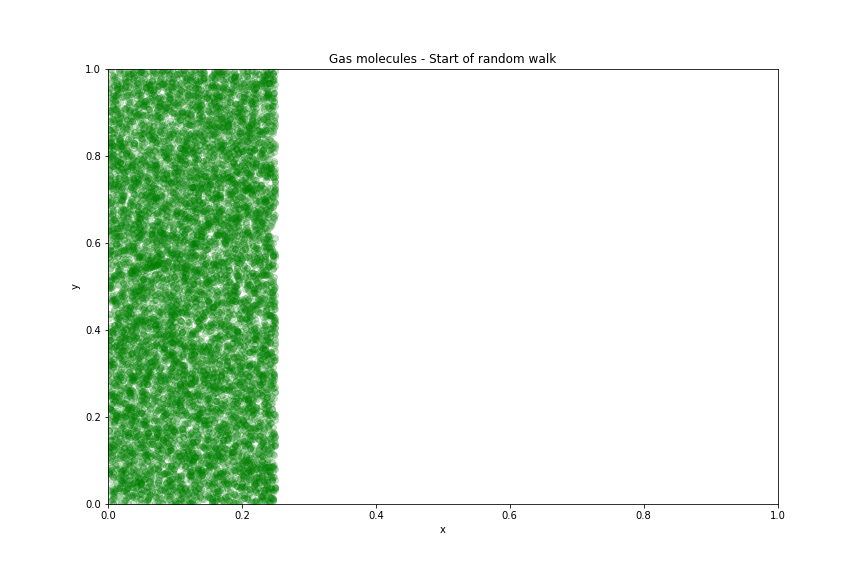
\includegraphics[width=18cm]{figures/final_start}
		\caption{Simulation Start Example - 10,000 molecules}
		\label{fig:simstart} % this gives the figure a unique name that you can refer to in the main text
	\end{figure}

	\clearpage
	
	By the end of the ten-thousand iterations, the molecules have had enough time to completely and uniformly fill the space, which you can clearly see in figure \ref{fig:simend}. Animated gif versions of these results can be found in the results folder.
	
	\begin{figure}[!hbt]
	\centering
	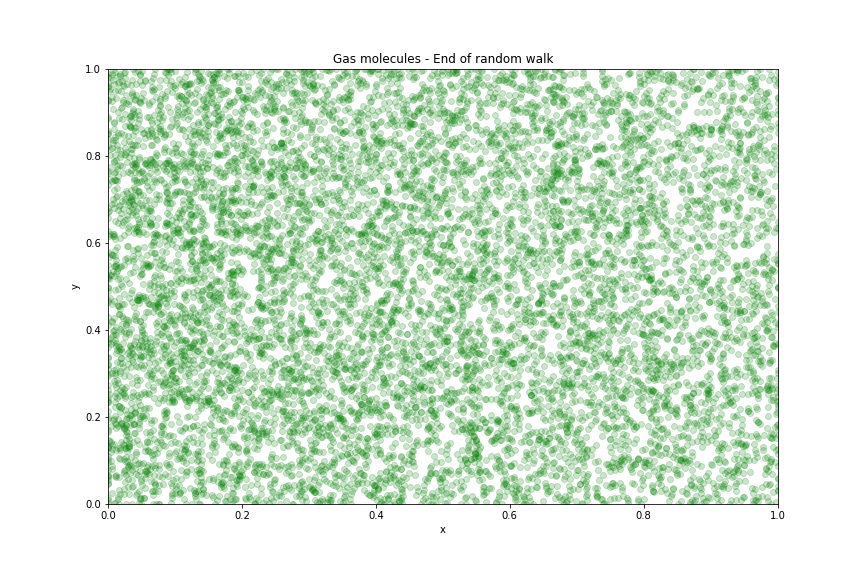
\includegraphics[width=18cm]{figures/final_end}
	\caption{Simulation End Example - 10,000 molecules}
	\label{fig:simend} % this gives the figure a unique name that you can refer to in the main text
	\end{figure}
	
	\section{Discussion}\label{conclusions}

	This was a really interesting project and it is easy to see how powerful computation simulations can be, even for simple problems. In the text book it states: \\
	
	Molecules tend to move randomly because of collisions and
	forces between molecules. We do not model collisions between particles in
	the random walk, but the nature of this walk, with random movements,
	simulates the effect of collisions. Therefore, the random walk can be
	used to model molecular motion in many simple cases. In particular, the
	random walk can be used to investigate how a quite ordered system,
	where one gas fills one half of a box, evolves through time to a more
	disordered system.\cite{Langtangen:2014:PSP:2676454}\\
	
	We think one of the most important aspects of this project is that it shows how a complex real life event can be simplified into a computer simulation while still providing useful results despite not fully modeling every aspect of gas molecules and their behavior. Such a translation is necessary because even though are computers today are very fast, they do not have unlimited resources. As you saw with the execution times, even a simple simulation such as this can take upwards of several minutes to complete. If you tried to model every aspect of the gas molecules and their behavior, the simulation would take much, much longer to complete. The end result however of uniformly filling a space would be the same. So in the end you must find a balance between simulation complexity and usefulness of the resulting data.

	\bibliographystyle{abbrv}
	\bibliography{library}
	
\end{document}